\chapter{Introduction}
\fixme{Need to include measuring properties as motivation and intro, so that it leads to glass paper}

\fixme{Need to include more about GPUs in motivation}

\fixme{Finish writing motivation}

\label{sec:intro}
\section{Scope}
The main goal of this thesis is to describe new techniques to bring movie production quality rendering into interactive applications.  The goal is to achieve photorealistic appearance as close as possible to the real world, while retaining the possibility for the user to interact with the simulation. In this thesis, we name these techniques "hybrid", as they combine techniques from the interactive world with accurate appearance models from physics and movie production pipelines.

Interactive realistic rendering applications are relevant in many fields, including
\begin{itemize}
\item 3D digital modeling and 3D printing,
\item Product development and visualization
\item Digital prototyping
\item Computer games and animation
\end{itemize}
In recent years, many advances have been made to achieve photorealistic quality in interactive applications,  but current techniques cannot achieve the photorealistic image quality that we see in movies. This thesis contributes with various techniques, exploring the area between interactive and real time rendering techniques (e.g. rasterization and interactive ray tracing), photorealistic rendering techniques (e.g. path tracing, hierarchical point cloud methods), and photorealistic appearance models (BRDFs and BSSRDFs, both analytical and measured). Our techniques, as most modern rendering techniques, are thought and developed to exploit the high throughput of graphic processing units (GPUs). Our contributions exploit both the long standing GPU hardware rasterization pipeline, but also focus on applications of the currently expanding field of interactive ray tracing. 

\section{Motivation}

\begin{figure}
\centering
	 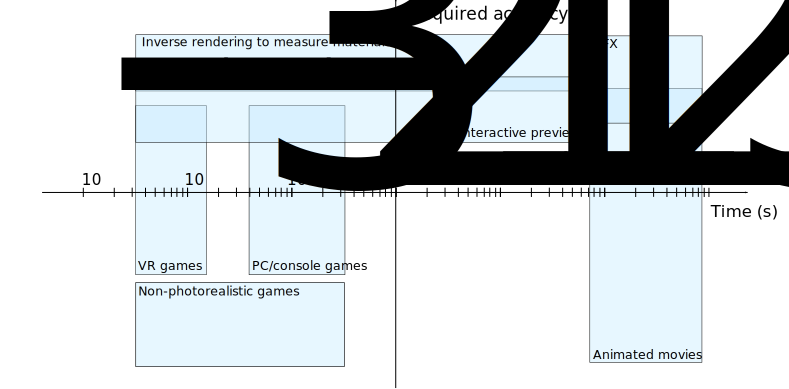
\includegraphics[width=\textwidth]{figures/main_diagram}  \\
\caption{Showing the continuum between interactive techniques, accurate techniques and photorealistic appearance.} 
\label{fig:main_diagram}
\end{figure}

\begin{itemize}
\item Realistic rendering - mention why it is important
\item Artistic based pipelines - challenges and why it is important to visualize data quickly
\item Big part of modern production - movie and games
\item Need for realistic models and visualization - effort on the modelling part, for phisically based models, and on the interaction part 
\item Tradeoffs are necessary, depending on the application
\item Noise versus converged vs simplified - do figure 
\item Spectrum of techniques
\item Refer to figure
\end{itemize}

In addition to the above motivations, we discuss three more detailed use cases in which there is a demand for improvements in photorealistic rendering techniques. These cases are not meant to be comprehensive of all applications in which interactive photorealistic rendering techniques are needed. However, they provide insights on possible industrial applications of the contributions in this thesis.

\subsection{3D printing}

\begin{itemize}
\item 3d printing: another group of applications where is important appearance
\item 3d printing; important to represent appearance faithfully
\item complicated materials
\item it has to be fast
\item More iterations, less discarded product
\item Color transformation during the process
\item Quality assurance as well
\item Material prediction 
\end{itemize}

The focus of the project goes towards a more strict integration of 3D printing processes and
digital image synthesis as a whole (The Digital-Physical Ecosystem). Our contribution to this
ecosystem will allow artists to work interactively on a 3D model while having a realistic overview
of the final appearance. This will allow more time for the artists to work faster, reducing
production times and waste of printing material.


\subsection{Architectural visualization}

\begin{itemize}
\item Light field visualization
\item Need for accurate materials
\item Also need for accurate visualization
\item Virtual reality
\item Accurate light simulation
\item Still interactive
\item Materials can be complicated to render accurately
\item Still convergence is acceptable
\end{itemize}

As we have discussed in Section TODO, many efforts have been made both in the offline and real time rendering community to achieve photorealistically accurate images. In the former community, more emphasis is put in achieving phisycal accuracy, while in the latter immediate feedback and performance are of foremost importance.

\subsection{Computer games and animation}
\begin{itemize}
\item Striving towards more realistic
\item Various interactive techniques
\item Volumetric techniques and interactive ray tracing
\item Rasteriation based usually
\item Relying on hardware
\item Relying on GPUs
\item Stricter requirements for performance
\item Simplification is more important than accuracy
\end{itemize}

In recent year, we have discussed how recent advantages in GPU power and interactive ray tracing are bringing phisically based rendering into the interactive domain. 

\section{Outcome}

During the three years period, we achieved a number of academic publications, reported at page TODO. In these publication, we managed to achieve a number of insights in the realm of computer graphics and material appearance. In particular, we created a range of techniques that can be readily applied to existing interactive applications. We believe we pushed the boundary on the degree of realism that can be achieved by modern GPUs on the same strict time constraints. 

In particular, papers TODO and TODO achieve in this by providing widely applicable caching in the realm of interactive subsurface scattering and global illumination. Some examples of the results achieved in these papers are reported in Figure TODO.

\section{Outline}

We report a list of all the contributions created during the course of the PhD studies at page TODO, including some unpublished notes, that we will refer mostly from Chapter TODO to provide additional details. All the various publications are available as appendices. 

We divide our thesis into four main chapters. In Chapter TODO, we first provide some background on some of the necessary foundations in radiometry, photorealistic appearance models and interactive rendering techniques. We will then provide in Chapter TODO an overarching literature review on the current efforts of the rendering community to achieve photorealistic interactive rendering, referring to the individual contributions for more detailed related work. In Chapter TODO, most importantly, we will go into more detail about the individual contributions and how each one of them contributes to reaching the outcome of the thesis. We will finally summarize our conclusions in Chapter TODO. 
